\documentclass[dvipdfmx]{jarticle}
<<<<<<< HEAD
\hoffset=-20mm
=======
\hoffset=-30mm
>>>>>>> dcc38b4 (241025-1746)
\pagestyle{empty}
\usepackage{tikz}
\usetikzlibrary{shapes,calc}
\begin{document}
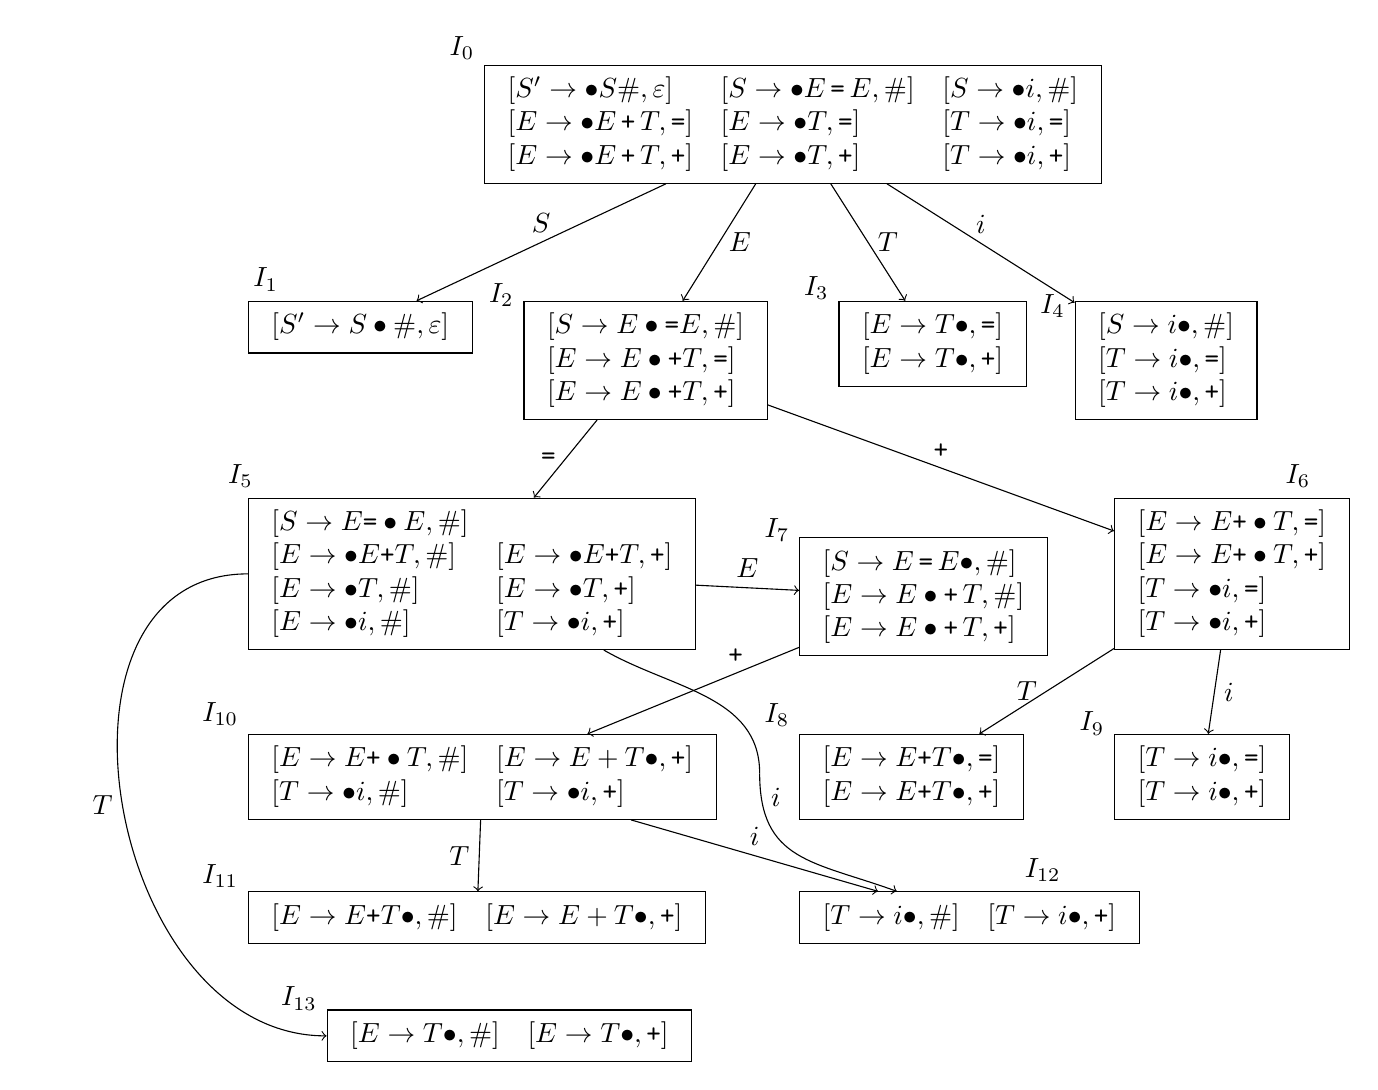
\begin{tikzpicture}
  \node[draw,rectangle,label=170:{$I_0$},anchor=north west] (I0) at (0,0) {
    $\begin{array}{lll}
      [S'\rightarrow\bullet S\#,\varepsilon] & [S\rightarrow\bullet E\,\texttt{=}\,E,\#] & [S\rightarrow\bullet i,\#]\\\relax
      [E\rightarrow\bullet E\,\texttt{+}\,T,\texttt{=}] & [E\rightarrow\bullet T,\texttt{=}] & [T\rightarrow\bullet i,\texttt{=}]\\\relax
      [E\rightarrow\bullet E\,\texttt{+}\,T,\texttt{+}] & [E\rightarrow\bullet T,\texttt{+}] & [T\rightarrow\bullet i,\texttt{+}]
    \end{array}$
  };

  \node[draw,rectangle,label=160:{$I_1$},anchor=north west] (I1) at (-3,-3) {
    $\begin{array}{l}
      [S'\rightarrow S\bullet\#,\varepsilon]
    \end{array}$
  };

  \node[draw,rectangle,label=160:{$I_2$},anchor=north west] (I2) at (0.5,-3) {
    $\begin{array}{l}
      [S\rightarrow E\bullet\texttt{=}E,\#]\\\relax
      [E\rightarrow E\bullet\texttt{+}T,\texttt{=}]\\\relax
      [E\rightarrow E\bullet\texttt{+}T,\texttt{+}]
    \end{array}$
  };

  \node[draw,rectangle,label=160:{$I_3$},anchor=north west] (I3) at (4.5,-3) {
    $\begin{array}{l}
      [E\rightarrow T\bullet,\texttt{=}]\\\relax
      [E\rightarrow T\bullet,\texttt{+}]
    \end{array}$
  };

  \node[draw,rectangle,label=160:{$I_4$},anchor=north west] (I4) at (7.5,-3) {
    $\begin{array}{l}
      [S\rightarrow i\bullet,\#]\\\relax
      [T\rightarrow i\bullet,\texttt{=}]\\\relax
      [T\rightarrow i\bullet,\texttt{+}]
    \end{array}$
  };

  \node[draw,rectangle,label=160:{$I_5$},anchor=north west] (I5) at (-3,-5.5) {
    $\begin{array}{ll}
      [S\rightarrow E\texttt{=}\bullet E,\#] & \\\relax
      [E\rightarrow \bullet E\texttt{+}T,\#] & [E\rightarrow\bullet E\texttt{+}T,\texttt{+}]\\\relax
      [E\rightarrow \bullet T,\#] & [E\rightarrow\bullet T,\texttt{+}]\\\relax
      [E\rightarrow \bullet i,\#] & [T\rightarrow\bullet i,\texttt{+}]
    \end{array}$
  };

  \node[draw,rectangle,label=60:{$I_6$},anchor=north west] (I6) at (8,-5.5) {
    $\begin{array}{l}
      [E\rightarrow E\texttt{+}\bullet T,\texttt{=}]\\\relax
      [E\rightarrow E\texttt{+}\bullet T,\texttt{+}]\\\relax
      [T\rightarrow \bullet i,\texttt{=}]\\\relax
      [T\rightarrow \bullet i,\texttt{+}]
    \end{array}$
  };


  \node[draw,rectangle,label=160:{$I_7$},anchor=north west] (I7) at (4,-6) {
    $\begin{array}{l}
      [S\rightarrow E\,\texttt{=}\,E\bullet,\#]\\\relax
      [E\rightarrow E\bullet\texttt{+}\,T,\#]\\\relax
      [E\rightarrow E\bullet\texttt{+}\,T,\texttt{+}]
    \end{array}$
  };

  \node[draw,rectangle,label=160:{$I_8$},anchor=north west] (I8) at (4,-8.5) {
    $\begin{array}{l}
      [E\rightarrow E\texttt{+}T\bullet,\texttt{=}]\\\relax
      [E\rightarrow E\texttt{+}T\bullet,\texttt{+}]
    \end{array}$
  };

  \node[draw,rectangle,label=160:{$I_9$},anchor=north west] (I9) at (8,-8.5) {
    $\begin{array}{l}
      [T\rightarrow i\bullet,\texttt{=}]\\\relax
      [T\rightarrow i\bullet,\texttt{+}]
    \end{array}$
  };

  \node[draw,rectangle,label=170:{$I_{10}$},anchor=north west] (I10) at (-3,-8.5) {
    $\begin{array}{ll}
      [E\rightarrow E\texttt{+}\bullet T,\#] & [E\rightarrow E+T\bullet,\texttt{+}]\\\relax
      [T\rightarrow \bullet i,\#] & [T\rightarrow\bullet i,\texttt{+}]
    \end{array}$
  };

  \node[draw,rectangle,label=175:{$I_{11}$},anchor=north west] (I11) at (-3,-10.5) {
    $\begin{array}{ll}
      [E\rightarrow E\texttt{+}T\bullet,\#] & [E\rightarrow E+T\bullet,\texttt{+}]
    \end{array}$
  };

  \node[draw,rectangle,label=30:{$I_{12}$},anchor=north west] (I12) at (4,-10.5) {
    $\begin{array}{ll}
      [T\rightarrow i\bullet,\#] & [T\rightarrow i\bullet,\texttt{+}]
    \end{array}$
  };

  \node[draw,rectangle,label=175:{$I_{13}$},anchor=north west] (I13) at (-2,-12) {
    $\begin{array}{ll}
      [E\rightarrow T\bullet,\#] & [E\rightarrow T\bullet,\texttt{+}]
    \end{array}$
  };

  \path[->] (I0) edge [above] node {$S$} (I1) (I0) edge [right] node {$E$} (I2)
            (I0) edge [right] node {$T$} (I3) (I0) edge [above] node {$i$} (I4);
  \path[->] (I2) edge [left] node {$\texttt{=}$} (I5) (I2) edge [above] node {$\texttt{+}$} (I6);
  \path[->] (I5) edge [above] node {$E$} (I7);
  \path[->] (I5) [out=180,in=180,looseness=1.2] edge [left] node {$T$} (I13);
  \path[-] (I5) [out=-30,in=90] edge (3.5,-9);
  \path[->] (3.5,-9) [out=270,in=160,looseness=1.25] edge [right,pos=0.1] node {$i$} (I12);
  \path[->] (I7) edge [above,pos=0.3] node {$\texttt{+}$} (I10);
  \path[->] (I6) edge [left] node {$T$} (I8) (I6) edge [right] node {$i$} (I9);
  \path[->] (I10) edge [above] node {$i$} (I12);
  \path[->] (I10) edge [left] node {$T$} (I11);
\end{tikzpicture}
\end{document}